% cases.tex - Case Study

\section{Case Study: Confining LLM-Generated Code}
\label{sec:cases}

The model is implemented in Jo\footnote{\url{https://jo-lang.org}}, a new
secure programming language whose broader design is described by Liu,
Blaudeau, and Lhot\'ak \cite{liu-jo-design}. %
This section uses Jo's surface syntax to show how the model applies to one
representative problem: safely executing code generated by a large language
model. %

Jo follows the object-capability discipline: dangerous operations are available
only through explicit capability values. %
The capability system adds static checking to that discipline. %
In Jo, \texttt{with} provides a capability value to a nested scope,
\texttt{allow} restricts which capabilities may be used in that scope, and
\texttt{receives} records an explicit capability requirement in a function
signature. %

\subsection{The Problem}

A platform may want generated code to analyze a user's data and emit a result,
while preventing it from reading arbitrary files, making network requests,
calling unrestricted tools, or accessing other users' data. %
The generated code is useful only if it can perform some actions, but those
actions must be narrow and reviewable. %

The naive design is to give generated code a broad runtime object, database
handle, or tool interface and rely on conventions inside the generated code. %
That is not confinement; it is trust. %
Even if the generated code is asked to use only one user's orders, a broad
database capability gives it more authority than the policy intends. %

\subsection{The Jo Design}

The framework is split into two libraries. %
The \emph{interface library} is the library against which generated code is
checked. %
It contains data types, capability declarations, and the expected entry-point
signature, but no FFI or other ambient authority. %
The \emph{runtime library} is trusted code. %
It may use FFI, databases, filesystem access, or other real services, but it
uses that authority only to construct the capability values supplied to the
generated code. %

\begin{figure}[t]
\centering
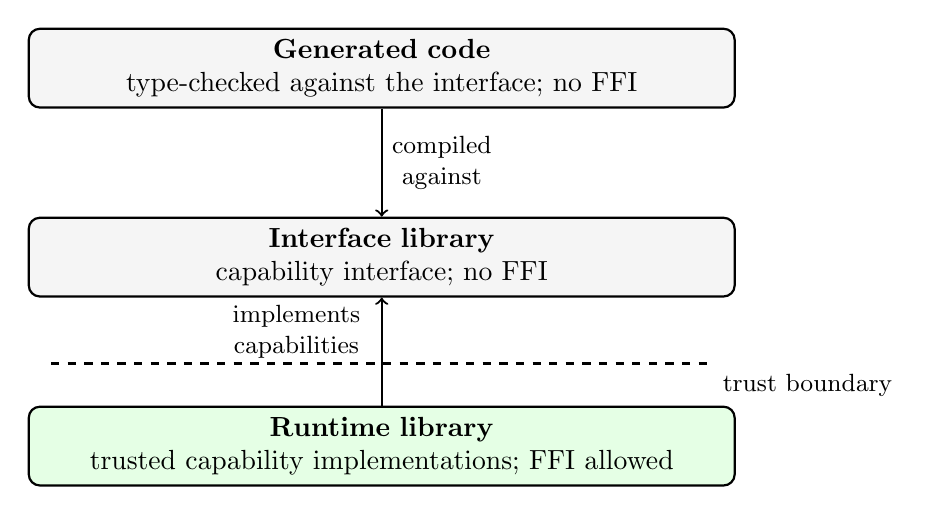
\begin{tikzpicture}[
  box/.style={draw, rounded corners, thick, align=center,
              text width=0.72\linewidth, minimum height=1.0cm},
  iface/.style={box, fill=gray!8},
  generated/.style={box, fill=gray!8},
  runtime/.style={box, fill=green!10},
  arrow/.style={->, thick},
  note/.style={font=\small, align=center}
]
  \node[generated] (ai) at (0,2.4)
    {\textbf{Generated code}\\type-checked against the interface; no FFI};
  \node[iface] (iface) at (0,0)
    {\textbf{Interface library}\\capability interface; no FFI};
  \node[runtime] (runtime) at (0,-2.4)
    {\textbf{Runtime library}\\trusted capability implementations; FFI allowed};

  \draw[dashed, thick] (-4.2,-1.35) -- (4.2,-1.35)
    node[note, below right]{trust boundary};
  \draw[arrow] (ai) -- node[note, right]{compiled\\against} (iface);
  \draw[arrow] (runtime) -- (iface);
  \node[note, left] at (-0.15,-0.95) {implements\\capabilities};
\end{tikzpicture}
\caption{Jo framework split for confining generated code. %
Only the runtime library below the trust boundary needs to be trusted.}
\label{fig:jo-framework-split}
\end{figure}

\autoref{fig:jo-framework-split} is the operational boundary. %
The interface library is the contract between the two sides. %
Generated code is not compiled against the runtime library, so it cannot name
its FFI-backed operations. %
Instead, generated code is compiled against the interface library, while the
trusted runtime library implements that interface and supplies concrete
capability values after generated code has been checked. %

In this example, the only input capability is \texttt{GetOrders}, a function
that returns orders for the current user, and the only output capability is
\texttt{IO.stdout}. %
The generated entry point must declare that it receives exactly those
capabilities. %

\begin{lstlisting}[style=pseudo]
param GetOrders: Int => List[Order]  // lastDays -> orders

defer def aiMain(): Unit receives GetOrders, IO.stdout
\end{lstlisting}

The framework constructs the actual capability values. %
It may internally use broad authority such as a database connection, the current
user identity, and a mutable output buffer. %
Those values remain in trusted code. %
The value given to generated code is an attenuated function that already
incorporates the user restriction. %

\begin{lstlisting}[style=pseudo]
def frameworkMain() =
  val db = connect("orders.db")
  val userId = currentUser()
  val restricted = (days: Int) => db.ordersFor(userId, days)

  val output: mutable.List[String] = []
  val buffer = (s: String) => output += s

  allow none in
    with GetOrders = restricted, IO.stdout = buffer in aiMain()
\end{lstlisting}

The generated program is checked against the interface it is allowed to use. %
It can read recent orders and write a summary, but it has no name for the
database, filesystem, network, or broader tool environment. %

\begin{lstlisting}[style=pseudo]
def aiMain(): Unit receives GetOrders, IO.stdout =
  val orders = GetOrders(30)
  summarize(orders)
\end{lstlisting}

\subsection{Why This Confines Authority}

The important point is where authority lives. %
The framework may possess broad authority, but it does not pass that authority
to generated code. %
Instead, it derives a narrower capability, \texttt{restricted}, and binds that
value as \texttt{GetOrders}. %
This is authority attenuation: the generated code can ask for orders, but only
through a function that has already fixed the user scope. %

\texttt{allow none} is also significant. %
It says that the body being run may not rely on ambient or already-in-scope
capabilities beyond those explicitly provided by the nested \texttt{with}. %
If generated code, or code reachable from it, requires some additional
capability, the compiler rejects the program. %
This gives the framework a static check that all direct and transitive
capability requirements have been mediated. %

This is the practical role of the captured-versus-caller-provided distinction in
the calculus. %
Trusted closures may capture broad internal state in order to build narrow
interfaces, but generated code receives only the caller-provided capabilities
listed in its signature and supplied at the call site. %
Captured authority is used to implement attenuation; caller-provided authority
is used to preserve control over invocation. %

The result is a design in which generated code can be useful without being
trusted with the whole runtime. %
It receives exactly the capabilities named by its interface, and the type system
checks that no additional capability is used. %
